\scanpage{12}
\mspage{9}
Then one sees that
\[
L^{n-i+\alpha}q_{i\alpha}:M^i-M^{2n-i+2\alpha}
\]
is zero on the $L^{\alpha'}P^{i-2\alpha'}$ for $\alpha'\neq\alpha$, and that on $L^\alpha P^{i-2\alpha}$, \deleted{it} its composite with
\[
P^{i-2\alpha}\xrightarrow{L^\alpha}L^\alpha P^{i-2\alpha}
\]
is none other than the isomorphism
\[
L^{n-i-2\alpha}:P^{i-2\alpha}\Rightarrow L^{n-i+2\alpha}P^{i-2\alpha}\subset M^{2n-i+2\alpha}.
\]
It follows at once that one has
\[
\pi_{i,\alpha}=L^\alpha w_{i-2\alpha}L^{n-i+\alpha}q_{i\alpha}=L^\alpha w_{i-2\alpha}L^{n-i+\alpha}(1-\sum_{\alpha'>\alpha}\pi_{i,\alpha'}
\tag{6.9}
\]
which indeed gives $\pi_{i\alpha}\in\mathcal E$. \deleted{This proves (iv).}
If $i<n$, one needs, also $\pi_{2n-i,\alpha}\in\mathcal E$. One
\deleted{It remains to prove \inserted{(iii)} $\Lambda\in\mathcal E$. It suffices to \deleted{\unsure{take}.} set
\[
q_{2n-i,\alpha}=1-\sum_{\alpha'>\alpha}\pi_{2n-i,\alpha'}
\]
and one then sees that
\[
\deleted{\unsure{L^{n-i+\alpha}}}L^\alpha q_{2n-i,\alpha}:M^{2n-i}-M^{2n-i+2\alpha}
\]}
deduces it for example from the formula
\[
\pi_{2n-i,\alpha}=L^{n-i}\pi_{i,\alpha}w_i\deleted{\unsure{\pi_{2n-i}}}
\tag{6.10}
\]
This proves \inserted{\figure{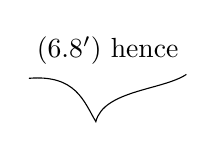
\begin{tikzpicture}[x=1cm,y=1cm]
\node at (0,.25) {$(6.8')$ hence};
\draw (-1,-.1) .. controls (-.4,-.05) and (-.3,-.4) .. (-.15,-.65) .. controls (-.05,-.25) and (.7,-.25) .. (1,-.05);
\end{tikzpicture}}} (iv). Remains : prove (iii) $\Lambda\in\mathcal E$.

Since one has
\[
\Lambda=\sum_{j,\alpha\,\deleted{\unsure{j\leq n}}}\deleted{\unsure{\Lambda}}\Lambda\pi_{j,\alpha}\quad\deleted{\unsure{+\sum_{\alpha\neq0}\Lambda}\quad\unsure{+\sum_{0\leq i\leq n}\pi_{i,0}\Lambda}}
\tag{6.11}
\]
it suffices to prove that $\Lambda\pi_{i\alpha}\deleted{\Lambda\pi_{i,\alpha}}\in\mathcal E$.
\mspage{11}
